	%% ++++++++++++++++++++++++++++++++++++++++++++++++++++++++++++
%% Hauptdatei, Wurzel des Dokuments
%% ++++++++++++++++++++++++++++++++++++++++++++++++++++++++++++

% Headerfeld, Typ des Dokumentes, einzubindende Packages.
% Hier bei Bedarf Änderungen vornehmen.
\documentclass
[   twoside=false,     % Einseitiger oder zweiseitiger Druck?
    fontsize=12pt,     % Bezug: 12-Punkt Schriftgröße
    DIV=15,            % Randaufteilung, siehe Dokumentation "KOMA"-Script
    BCOR=17mm,         % Bindekorrektur: Innen 17mm Platz lassen. Copyshop-getestet.
%    headsepline,
    headsepline,  % Unter Kopfzeile Trennlinie (aus: headnosepline)
    footsepline,  % Über Fußzeile Trennlinie (aus: footnosepline)
    open=right,        % Neue Kapitel im zweiseitigen Druck rechts beginnen lassen
    paper=a4,          % Seitenformat A4
    abstract=true,     % Abstract einbinden
    listof=totoc,      % Div. Verzeichnisse ins Inhaltsverzeichnis aufnehmen
    bibliography=totoc,% Literaturverzeichnis ins Inhaltsverzeichnis aufnehmen
    titlepage,         % Titelseite aktivieren
    headinclude=true,  % Seiten-Head in die Satzspiegelberechnung mit einbeziehen
    footinclude=false, % Seiten-Foot nicht in die Satzspiegelberechnung mit einbeziehen
    numbers=noenddot   % Gliederungsnummern ohne abschließenden Punkt darstellen
]   {scrreprt}         % Dokumentenstil: "Report" aus dem KOMA-Skript-Paket

\usepackage[active]{srcltx}
\overfullrule=2cm
%\usepackage[activate=normal]{pdfcprot} % Optischer Randausgleich -> pdflatex!
\usepackage{ifthen}
\usepackage[ngerman]{babel}   % Neue Deutsche Rechtschreibung
%\usepackage[latin1]{inputenc} % Zeichencodierung nach ISO-8859-1
\usepackage[utf8]{inputenc}   %	Zeichencodierung nach UTF-8 (Unicode)
\usepackage[T1]{fontenc}
\usepackage{graphicx}
%\usepackage{ae} % obsolet und durch lmodern ersetzt
\usepackage{lmodern}
\usepackage{listings}
\usepackage[T1]{url}
\usepackage{amsthm}
\usepackage{amsmath}
\usepackage{graphicx}
\RequirePackage{scrlfile}
\ReplacePackage{scrpage2}{scrlayer-scrpage}
% old: \usepackage[automark]{scrpage2}
\usepackage[automark]{scrlayer-scrpage}
\usepackage{setspace}
% Farben und so 
\usepackage{xcolor}
%\usepackage[first,light]{draftcopy} % Für Probedruck
\usepackage[plainpages=false,pdfpagelabels,hypertexnames=false]{hyperref}



%% UNIX 
\makeatletter
\DeclareOldFontCommand{\rm}{\normalfont\rmfamily}{\mathrm}
\DeclareOldFontCommand{\sf}{\normalfont\sffamily}{\mathsf}
\DeclareOldFontCommand{\tt}{\normalfont\ttfamily}{\mathtt}
\DeclareOldFontCommand{\bf}{\normalfont\bfseries}{\mathbf}
\DeclareOldFontCommand{\it}{\normalfont\itshape}{\mathit}
\DeclareOldFontCommand{\sl}{\normalfont\slshape}{\@nomath\sl}
\DeclareOldFontCommand{\sc}{\normalfont\scshape}{\@nomath\sc}
\makeatother

%% 

% Tiefe der Kapitelnummerierung beeinflussen
\setcounter{secnumdepth}{3} % Tiefe der Nummerierung
\setcounter{tocdepth}{3}    % Tiefe des Inhaltsverzeichnisses

% Datum anpassen
\newcommand{\leadingzero}[1]{\ifnum #1<10 0\the#1\else\the#1\fi}
\renewcommand{\today}{\leadingzero{\day}.\leadingzero{\month}.\the\year}     % DD.MM.YYYY

% Hier in die zweite geschweifte Klammer jeweils
% die persoenlichen Daten und das Thema der Arbeit eintragen:
\newcommand{\artderausarbeitung}{Finales Review Document}
\newcommand{\namedesautorsI}{P.~Augustin, C.~Juin, }
\newcommand{\namedesautorsII}{G.~Lehmann, A.~Schmidt, R.~Schöne}
\newcommand{\themaderarbeit}{RION  Package-Manager}
\newcommand{\xRION}{\RION}
%% Das passt schon so 
\newcommand{\namedesautors}{\namedesautorsI \namedesautorsII}

% PDF Metadaten definieren
\hypersetup{
   pdftitle={\themaderarbeit},
   pdfsubject={\artderausarbeitung},
   pdfauthor={\namedesautors},
   pdfkeywords={\artderausarbeitung; TU-Ilmenau}}


% Abkürzungsverzeichnis beeinflussen. Hier nichts ändern!
\usepackage[intoc]{nomencl}
  \AtBeginDocument{\setlength{\nomlabelwidth}{.25\columnwidth}}
  \let\abbrev\nomenclature
  \renewcommand{\nomname}{Abkürzungsverzeichnis und Formelzeichen}
  \renewcommand{\nomlabel}[1]{#1 \dotfill}
  \setlength{\nomitemsep}{-\parsep}
  \makenomenclature

\usepackage[normalem]{ulem}
  \newcommand{\markup}[1]{\textbf{#1}}

% Seitenlayout festlegen. Hier nichts ändern!
\pagestyle{scrplain}
\ihead[]{\headmark}
\ohead[]{\pagemark}
\chead[]{}
\ifoot[]{}
\ofoot[]{\scriptsize \artderausarbeitung\ - \namedesautors}
\cfoot[]{}
\renewcommand{\titlepagestyle}{scrheadings}
\renewcommand{\partpagestyle}{scrheadings}
\renewcommand{\chapterpagestyle}{scrheadings}
\renewcommand{\indexpagestyle}{scrheadings}



% Abschnittsweise Nummerierung anstatt fortlaufend. Hier nichts ändern!
\makeatletter
\@addtoreset{equation}{chapter}
\@addtoreset{figure}{chapter}
\@addtoreset{table}{chapter}
\renewcommand\theequation{\thechapter.\@arabic\c@equation}
\renewcommand\thefigure{\thechapter.\@arabic\c@figure}
\renewcommand\thetable{\thechapter.\@arabic\c@table}
\makeatother
\renewcommand*{\pagedeclaration}[1]{\unskip, \hyperpage{#1}}

% Quelltextrahmen, klein. Hier nichts ändern!
\newsavebox{\inhaltkl}
\def\rahmenkl{\sbox{\inhaltkl}\bgroup\small\renewcommand{\baselinestretch}{1}\vbox\bgroup\hsize\textwidth}
\def\endrahmenkl{\par\vskip-\lastskip\egroup\egroup\fboxsep3mm%
\framebox[\textwidth][l]{\usebox{\inhaltkl}}}

% Quelltextrahmen, normale Groesse. Hier nichts ändern!
\newsavebox{\inhalt}
\def\rahmen{\sbox{\inhalt}\bgroup\renewcommand{\baselinestretch}{1}\vbox\bgroup\hsize\textwidth}
\def\endrahmen{\par\vskip-\lastskip\egroup\egroup\fboxsep3mm%
\framebox[\textwidth][l]{\usebox{\inhalt}}}


% Sonstige Befehlsdefinitionen hier ablegen.
\newcommand{\entspricht}{\stackrel{\wedge}{=}}
\newcommand{\quotes}[1]{\glqq#1\grqq{}}
\newcommand{\x}{X-FAB} % sry :)
\newcommand{\e}{RION} % well
\newcommand{\Linux}{GNU/Linux}
\makenomenclature


% Tabellenspaltendefinitionen mit fester Breite --> somit Zeilenumbruch innerhalb einer Zelle möglich
% aus http://www.torsten-schuetze.de/tex/tabsatz-2004.pdf
\usepackage{array, booktabs}
\newcolumntype{f}{>{$}l<{$}}
\newcolumntype{n}{>{\raggedright}l}
\newcolumntype{N}{>{\scriptsize}l}
\newcolumntype{v}[1]{>{\raggedright\hspace{0pt}}m{#1}}
\newcolumntype{V}[1]{>{\scriptsize\raggedright\hspace{0pt}}m{#1}}
\newcolumntype{Z}[1]{>{\raggedright\centering}m{#1}}
\newcolumntype{k}[1]{>{\raggedright}p{#1}}
% ergibt Tabllenspalte fester Breite, linksbündig
% Umbruch innerhalb der Zelle mit \\, neue Tabellezeile mit \tabularnewline
% \addlinespace für Gruppentrennung (aus \texttt{booktabs.sty})


\begin{document}
\onehalfspacing

\begin{titlepage}
	\centering
	{\Large \textsc{Technische Universität Ilmenau}}\\[3ex]
	{\Large Rechnerarchitekturen und Eingebettete Systeme}\\[3ex]
	\vfill
	{\Large \textbf{\artderausarbeitung}}\\[4ex]
	{\large \textbf{\themaderarbeit}}\\[5ex]
	%{\large \textbf{\xRION}}\\[5ex]
	\vfill
	\begin{tabular}{rl}
		\hline\\
		vorgelegt von:          & \quad \namedesautorsI\\[1,5ex]
										       & \quad \namedesautorsII\\[1,5ex]
		eingereicht am:         & \quad 
		\today \\[1,5ex]
		Fachgebiet:            & \quad Rechnerarchitekturen und Eingebettete Systeme\\[0,5ex]
								& \quad Institut für Mikroelektronik- und Mechatronik-System\\[1,5ex]
		Betreuer:            	& \quad Georg Gläser, Andreas Becher \\[1,5ex]
		Seminarleiter           & \quad Prof. Armin Zimmermann \\[1,5ex]	
	\end{tabular}
	\vfill
	
    


\end{titlepage}
%%% ++++++++++++++++++++++++++++++++++++++++++++++++++++++++++++
%% Zusammenfassung, Abstract
%% ++++++++++++++++++++++++++++++++++++++++++++++++++++++++++++


\renewcommand{\abstractname}{Kurzfassung}
\begin{abstract}
	\begin{center}
		X-FAB bietet eine Fülle an unterschiedlichen Technologien für diverse und auch
        spezifische Anwendungsmärkte an. Um Packete für das Process Design Kit verwalten zu können soll ein Package-Manager mit dem Namen RION geschaffen werden
	\end{center}
\end{abstract}

% Inhaltsverzeichnis
\cleardoublepage % Seitenumbruch erzwingen vor Änderung des Nummerierungsstils
\pagenumbering{roman} % Nummerierung der Seiten ab hier: i, ii, iii, iv...
\pagestyle{scrheadings} % Ab hier mit Kopf- und Fusszeile
\tableofcontents

% Die einzelnen Kapitel
\cleardoublepage % Seitenumbruch erzwingen vor Änderung des Nummerierungsstils
\pagenumbering{arabic} % Nummerierung der Seiten ab hier: 1, 2, 3, 4...

%%% Content %%%
\part*{Reviewdokument}

%% Pages
\chapter{Zweck des Systems}

\section{Anwendungsbereiche}
Der vorliegende Package-Manager richtet sich an Entwickler, sowie Kunden und Entwickler der X-FAB. \\
RION soll die technischen Grundanforderungen zur PDK-Installation auf Kundenseite auf ein Minimum begrenzen. Durch entsprechende PDK-Paketinformationen und eine Plausibilitätsprüfung dieser, durch RION \quotes{(rion check)}, sollen Fehler bei der Installation von PDK-Paketen verhindert werden. Diese könnten im schlimmsten Fall zu einer Fehlfunktion des Halbleiterchips führen.

\section{Zielgruppe}
Die Zielgruppe umfasst alle Kunden der X-FAB.


\chapter{Zielbestimmungen}

RION ist ein Package-Manager zum suchen, installieren, aktualisieren und verwalten von Packages für das Process Design Kit (PDK). Die Pakete für RION werden von der Serverseite INOR verwaltet.

\section{Problemstellung}
Zur Zeit werden Packages manuell von einem Webinterface heruntergeladen. Sie werden manuell installiert und aktualisiert. Dieser jetzige Weg ist jedoch unübersichtlich, fehleranfällig, inkonsistent, kostet sehr viel Zeit und erfordert sehr viel manuelle Arbeit, sowohl server- als auch clientseitig. Daher soll dieser Prozess durch Verwendung von RION, clientseitig für X-Fab-Kunden, und INOR, serverseitig für X-FAB-Entwickler, vereinfacht und automatisiert werden.

\section{Musskriterien}
\subsection{Funktionalität}
\begin{itemize}
		\item INOR muss die Packages serverseitig über eine Datenbank in Form von Archiven zur Verfügung stellen.
		\item RION muss eine Liste der auf dem Server vorliegenden Pakete herunterladen und durchsuchen können.
		\item RION muss Pakete installieren können. Dabei müssen auch ältere Versionen des Paketes zugänglich gemacht werden können.
		\item RION muss installierte Pakete aktualisieren können. In diesem Kontext bedeutet das, dass die neuere Version des Paketes parallel zur Alten zu installiert wird.
		\item RION muss installierte Pakete entfernen können.
\end{itemize}

\subsection{Interaktion}


\begin{itemize}
	\item Dem Benutzer muss ein CLI zur Verfügung stehen.
\end{itemize}

\section{Wunschkriterien}
\begin{itemize}
	\item INOR soll Pakete signieren.
	\item INOR soll Hashwerte von Paketen anfertigen und an RION übermitteln können.
	\item RION soll nach dem Herunterladen, aber vor der Installation, Pakete auf ihre Signatur, sowie auf ihren korrekten Hashwert überprüfen.

\end{itemize}

\chapter{Grobentwurf}
\\[\intextsep]
\begin{minipage}{\linewidth}
\centering%
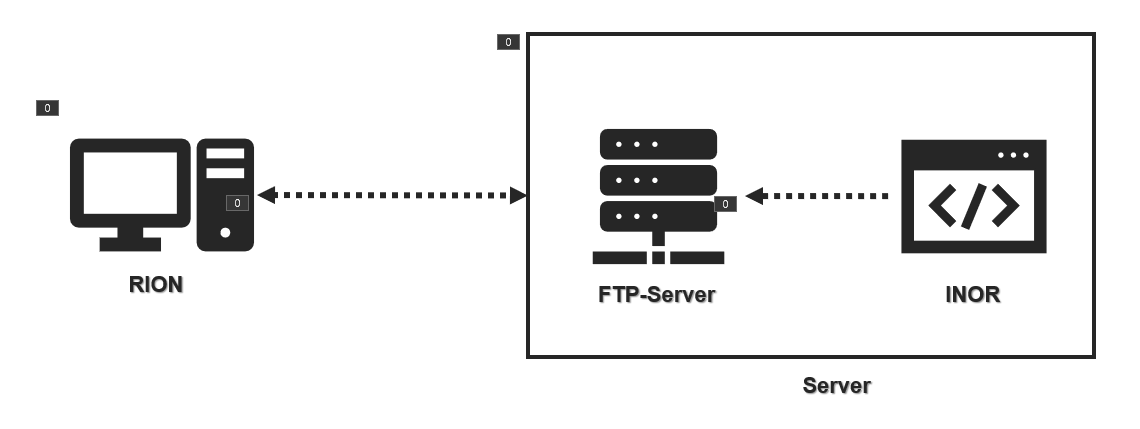
\includegraphics[width=0.8\linewidth,clip=]{./img/Img1.jpg}%
\label{fig:Image 1}%
\end{minipage}
\\[\intextsep]

Das Programm arbeitet prinzipiell mit drei Komponenten. Zum einen gibt es den
Packagemanger RION. Dieser läuft auf dem jeweiligen Endgerät (Client), der Pakete sucht,
installiert, aktualisiert, entfernt und verwaltet. Hierzu werden mehrere Datenbanken
verwendet. Darunter eine Datenbank, die eine Liste aller installierten Pakete enthält und eine
Andere, mit einer Liste der Namen aller verfügbaren Pakete, sowie deren Metadaten und die
Namen der notwendigen Abhängigkeiten. \\


Die Pakete sowie die zweite genannte Datenbank können von einem FTP-Server über eine
verschlüsselte ftps-Verbindung abgerufen werden. Hierzu wird das Programm pyftpdlib,
welches unter anderem virtuelle Nutzer zur Verfügung stellt, die zum Rechtemanagement
verwendet werden. (Dieses Programm wird nicht nicht von uns entwickelt.)
\\

Die Daten für den FTP-Server sowie die Konfiguration der Rechteverwaltung werden durch
die Dritte Komponente INOR zur Verfügung gestellt. Welche diesen Vorgang durch einige
Funktionen erleichtert bzw. automatisiert. INOR befindet sich dabei auf dem selben Server,
wie der FTP-Server.\\   
\chapter{UML}

\section{Weitere Sinnlose Diagramme}
\begin{minipage}{\linewidth}
\centering%
\includegraphics[width=0.8\linewidth,clip=]{./img/blödsinn.png}%
\captionof{figure}{blödsinn}%
\label{fig:blödsinn}%
\end{minipage}
\vspace{10px}

\section{Doxygen}

Die Ausführliche von Doxygen generierte Dokumentation ist im Anhang zu finden.




\chapter{Bug Report}
\section{Unclear error message}
\begin{itemize}
    \item Anpassen der Error Messages.
    \begin{itemize}
        \item alt: Missing Input
        \item neu: Missing login credentials. Please enter them in the config file or with "rion login" 
    \end{itemize}
    \item: GitHub Issue #23:\url{https://github.com/Riffecs/rion/issues/23}
    \item Status: Fixed, Closed
\end{itemize}

\section{Wrong Syntax}
\begin{itemize}
    \item Erlauben von Sonderzeichen bei Passwörtern.
    \begin{itemize}
        \item alt: Keine Sonderzeichen erlaube
        \item neu: erlaubt Sonderzeichen
    \end{itemize}
    \item: GitHub Issue #20:\url{https://github.com/Riffecs/rion/issues/20}
    \item Status: Fixed, Closed
\end{itemize}

\section{Delete the name from the licence}
\begin{itemize}
    \item Entfernen der Namen.
    \begin{itemize}
        \item alt: Namen stehen in der Lizenz
        \item neu: Schaffung eines Templates zur Entfernung der Namen
    \end{itemize}
    \item: GitHub Issue #16:\url{https://github.com/Riffecs/rion/issues/16}
    \item Status: Fixed, Closed
\end{itemize}

\section{Error: Invalid Version}
\begin{itemize}
    \item Prüfen von Versionsnummern.
    \begin{itemize}
        \item alt: Durch eine Diskrepanz in der Versionsnummer stürzte Rion immer ab
        \item neu: Entfernen der Versionsprüfung
    \end{itemize}
    \item: GitHub Issue #16:\url{https://github.com/Riffecs/rion/issues/16}
    \item Status: Fixed, Closed
\end{itemize}

Alle Issues können im Git im Reiter Issue \footnote{\url{https://github.com/Riffecs/rion/issues?q=is\%3Aissue}} eingesehen werden.
\chapter{Testszenarien}

\section{RION}

\begin{itemize}
	\item[T0110] \textit{Installation:} Der Nutzer installiert mit \quotes{rion install \textit{Packagename}} ein Paket. Das Paket wird, inklusive eventueller Abhängigkeiten, installiert. Skripte (Post-Install-Prozessierung) werden erfolgreich ausgeführt.
	\item[T0120] \textit{Suchen:} Der Nutzer sucht mit \quotes{rion search \textit{text}} ein Paket und bekommt eine Liste von passenden Paketen, inklusive einer kurzen Beschreibung derer, ausgeben.
	\item[T0130] \textit{Information:} Der Nutzer sucht mit \quotes{rion info \textit{Packagename}} Informationen zu einem Paket und bekommt diese detailliert zu einem Paket ausgeben.
	\item[T0140] \textit{Aktualisieren:} Der Nutzer aktualisiert mit \quotes{rion update} alle installierten Pakete. Diese werden aktualisiert. Er aktualisiert mit \quotes{rion upgrade \textit{Packagename}} ein bestimmtes Paket, welches nun aktualisiert wird.
	\item[T0150] \textit{Entfernen:} Der Nutzer entfernt mit \quotes{rion remove \textit{Packagename/s}} ein oder mehrere Pakete, welche dadurch deinstalliert werden.
	\item[T0160] \textit{Anleitung:} Der Nutzer schreibt \quotes{man rion}, worauf ihm die Manpage zu RION angezeigt wird.
	\item[T0170] \textit{Installierte Pakete listen:} Der Nutzer gibt \quotes{\textit{rion list (package\_name\_pattern)}} ein. Er erhält Liste aller installierten Pakete, bzw. aller installierten Funktionen eines Paketes.
	\item[T0180] Die Repositories, auf die RION zugreift, können mit einem config file angepasst werden.
	\item[T0190] RION kann mehrere virtuellen Umgebungen verwalten.
	\item[T0111] RION kann mit 	\quotes{rion check (\textit{Packagename (Packageversion)})} überprüfen, ob bestimmte oder alle installierten Pakete noch korrekt installiert sind.
	\item[T0121] RION kann mit \quotes{rion update} die lokale Datenbank aktualisieren.
	\item[T0131] RION kann sich mit \quotes{rion auth -u >>USER<< -p >>PWD<<} anmelden. RION kann sich auch über einen config file (nur für den Ersteller lesbar) anmelden. Sollte keine Anmeldung vorliegen, fragt RION beim ersten Aufruf nach den Anmeldedaten.


\end{itemize}

\section{INOR}

\begin{itemize}
	\item[T0210] \textit{Paket hinzufügen:} Der Nutzer fügt mit \quotes{inor add \textit{Packagename Packagefile}} ein Paket zur Datenbank hinzu, welches noch nicht in der Datenbank ist. Daraufhin befindet es sich in der Datenbank. Abhängigkeiten wurden berücksichtigt.
	\item[T0220] \textit{Neue Version hinzufügen:} Der Nutzer fügt mit \quotes{inor update \textit{Packagename Packageversion Packagefile}} eine neue Version eines vorhandenen Paketes zur Datenbank hinzu. Es befindet sich daraufhin in der Datenbank.
	\item[T0230] \textit{Beschreibung hinzufügen:} Der Nutzer fügt mit \quotes{inor describ \textit{Packagename}} jene Beschreibung zu einem Paket hinzu, die beim Suchen durch RION abgerufen wird. Die Beschreibung ist nun abrufbar.
	\item[T0240] \textit{Lizenz:} Der Nutzer fügt mit \quotes{rion install \textit{Packagename}} Lizenzinformation hinzu.
	\item[T0250] \textit{Paket entfernen:} Der Nutzer entfernt mit \quotes{inor remove \textit{Packagename}} alle Versionen eines Paketes aus der Datenbank oder er kann mit \quotes{inor remove \textit{Packagename Versionsnummer}} eine bestimmte Version eines Paketes aus der Datenbank entfernen.
	\item[T0260] \textit{Paket signieren:} Der Nutzer signiert mit \quotes{inor sign} alle installierten Pakete in der Datenbank oder er signiert mit \quotes{rion sign \textit{Packagename (Versionsnummer)}} ein bestimmtes Paket oder auch nur eine bestimmte Version eines Paketes. Die spezifizierten Pakete sind daraufhin signiert.
	\item[T0270] \textit{Pakete publizieren:} Der Nutzer schaltet mit \quotes{textit{inor publish Packagename (Packageversion)}} alle spezifizierten Pakete für RION frei. Daraufhin kann RION auf die spezfizierten Pakete zugreifen.
	\item[T0280] \textit{Pakete publizieren:} Der Nutzer sperrt mit \quotes{\textit{inor unpublish Packagename (Packageversion)}} alle spezifizierten Pakete für RION. Daraufhin kann RION auf die spezfizierten Pakete nicht mehr zugreifen.
	\item[T0290] \textit{Anleitung:} Der Nutzer schreibt \quotes{man inor}, worauf ihm die Manpage zu RION angezeigt wird.
\end{itemize}

\chapter{Testfälle}

\section{Komponenten Test}
\begin{itemize}
    \item \_\_init\_\_.py : erstellt einen Handler bleibt danach inaktiv bis Beendigung
    \item \_\_main\_\_.py : erstellt einen Handler bleibt danach inaktiv bis Beendigung
    \item database.py : erstellt einen Handler bleibt danach inaktiv bis Beendigung
    \item errors.py : erstellt einen Handler bleibt danach inaktiv bis Beendigung
    \item ftp.py : erstellt einen Handler bleibt danach inaktiv bis Beendigung
    \item helper.py : erstellt einen Handler bleibt danach inaktiv bis Beendigung
    \item rion.py : erstellt einen Handler bleibt danach inaktiv bis Beendigung
\end{itemize}


\section{Blackbox}
\begin{itemize}
    % \item $\rightarrow$ Vom video herziehen
    \item Uninstall funktion rion $\rightarrow$ deinstalliert rion 
    \item Man rion $\rightarrow$ lädt und zeigt die man page
    \item rion Login funktion $\rightarrow$ user eingeloggt
    \item rion Update funktion $\rightarrow$ rion aktualisiert
    \item rion remove funktion $\rightarrow$ packet entfernt
    \item rion upgrade funktion $\rightarrow$ packet aktualisiert
    \item ion seach funktion $\rightarrow$ zeigt packete mit dem eingegebenen Namen/Flags
\end{itemize}

\chapter{Kritische Betrachtung}

Abschließend ergaben sich aus der Arbeit am Projekt „RION“ vielschichtige Erkenntnisse, die retrospektiv betrachtet werden müssen.
Idealerweise sollten dem Projekt gewisse Parameter in der Vorgehensweise vorausgesetzt sein, die für den Erfolg der Durchführung unseres Erachtens unabdingbar sind. Dazu gehören als Mindestvoraussetzung die termingerechte Gruppenbildung und eine grundsätzliche Themenaffinität der Gruppenmitglieder. Einerseits, um den vorgeschriebenen Zeitrahmen optimal nutzen zu können und andererseits das Potenzial an Motivation und Kompetenzen in dem höchsten Grade ausschöpfen zu können. Also braucht es eine gewisse sinnhafte Kompatibilität des Teams untereinander. Hierzu zählt jedenfalls ein annähernd gleicher Wissensstand bei grundlegenden projektimmanenten Inhalten. Je weniger fachlicher Aufholbedarf untereinander ausgeglichen werden muss, desto effizienter der Fortschritt der Gemeinschaftsarbeit. Hierbei wird das gegenseitige profitieren und dazulernen auf fachfremden Gebieten der Teammitglieder aus unterschiedlichen Bereichen nicht grundsätzlich in Abrede gestellt. Wohlgemerkt gilt die Kritik einem mangelnden gemeinsamen Grundwissen. Fachlich betrachtet meint dies bei dem vorliegendem Projekt, dass sich alle Teilnehmer mit der jeweils angewandten Programmiersprache, der UML, dem Zielbetriebssystem, dem genutzten Vorgehensmodell und sowie grundlegenden Programmierparadigmen und der OOP auskennen müssten.
Von größter Bedeutung für Erfolg oder Misserfolg des Projektes sind auch soziale Komponenten. Eine unbedingte Kommunikations- und Kooperationsbereitschaft muss zwingend kleinster gemeinsamer Nenner im Team sein. Selbst fruchtbringende Alleingänge müssen dem Team transparent und diskutierbar gemacht werden. Teamwork muss Priorität haben, um gemeinsame Fortschritte zu generieren. Dazu bedarf es des unumstößlichen Willens eigene Fähigkeiten in den Dienst des Teams zu stellen und sich nicht nur selbst vordergründig profilieren zu wollen. Dass das Team nach außen hin als solches auftritt, muss dabei selbstverständlich sein.
Zur Organisation der Teilnehmer ist es zwingend angeraten, dass zentrale Plattformen gewählt, bedient und regelmäßig und zuverlässig besucht werden – eine Grundkomponente effektiver Kommunikation!
Ideal sollte schließlich das Ergebnis zielorientiert zu den gewünschten Ergebnissen führen.\\
In erster Linie müssen die Kundenanforderungen bedarfsgerecht erfüllt worden sein. Das heißt das Ergebnis des Projektes muss voll funktionsfähig sein, was in diesem Fall scheiterte. Wünschenswert waren auch mögliche zusätzlich eingebrachte Funktionen, die im Verlauf des Projektes ebenfalls angedacht worden waren.
Termintreu hätten abschließend alle Tests bestanden werden müssen und nonfunktionale Anforderungen übertroffen werden können. Damit sind zum Beispiel Fragen von Sicherheit, Leistungsfähigkeit, Robustheit etc. gemeint.
In vorliegendem Fall konnten viele dieser Ansprüche aus verschiedensten Gründen nicht realisiert werden, unter anderem deshalb, da voraussetzende Parameter nicht gegeben waren.



%% Syntax
% This file is a ghost. Only abbreviations for foreign words or new words are stored here. Nothing more
\makenomenclature
\nomenclature{RION}{Packagemanager und Schnittstelle für die Paketverwaltung zwischen X-FAB-Server und Client}

\nomenclature{X-FAB}{Die X-FAB ist ein Anbieter für Halbleitertechnologien, welcher sowohl die Fertigung als auch Designunterstützung für Kunden anbietet, die gemischt analog-digitale integrierte Schaltkreise (ICs) entwickeln. Die X-FAB bietet eine Reihe an unterschiedlichen Technologien für diverse und auch
spezifische Anwendungsmärkte an.}

\nomenclature{INOR}{Serverseitiges BackEnd bei der X-FAB.}

\nomenclature{Pakete/Packages}{Datenbündel, die als solches eine Funktion haben. Hiermit sind die Pakete auf den X-FAB-Servern gemeint.}

\nomenclature{pyftpdlib}{FTP-Server-Implementation für Python}

\nomenclature{Python}{Programmiersprache: \url{https://www.python.org/}}

\nomenclature{CLI}{Ein \texttt{C}ommand \texttt{L}ine \texttt{I}nterface ist eine Schnittstelle, die es dem Nutzer erlaubt, Textbefehle an ein Programm zu übermitteln. Betriebssysteme, darunter GNU/Linux stellen hierfür eine sogenannte Shell, wie zum Beispiel Bash, Dash oder ZSH, zur Verfügung, auf welche man mit einem Terminal zugreifen kann.}

\nomenclature{Manpage}{Eine Hilfeseite für installierte Programme unter Unix-artigen Systemen, auf der für gewöhnlich Befehle, Flags und Hinweise zur Benutzung eines Programms verzeichnet sind. Darauf zugegriffen wird mit \texttt{man >>name<<}.}

\nomenclature{pip}{Python Package-Manager: \url{https://pypi.org/project/pip/}}

\nomenclature{PDK}{Ein PDK ist eine komplexe Sammlung von technologiespezifischen Daten für den aufwändigen und
relativ teuren Entwurf von anwendungsspezifischen integrierten Schaltkreisen.}

\nomenclature{PyPi}{Pypi ist eine Softwaresammlung, durch die Pythonpackages via pip heruntergeladen werden können.}

\printnomenclature
%%% Ende %%%

\appendix
%\part*{Anhang}


% Anahng
%%% ++++++++++++++++++++++++++++++++++++++++++++++++++++++++++++
%% Anhang: Literaturverzeichnis
%% ++++++++++++++++++++++++++++++++++++++++++++++++++++++++++++


% Mit dem Befehl \nocite werden auch nicht im Text zitierte
% aus der Literaturdatenbank mit in das Literaturverzeichnis aufgenommen.
% Ein "\nocite{*}" übernimmt ungeprüft die komplette Datenbank.
%\nocite{*}

\cleardoublepage
\nocite{*}
\ihead[]{Literaturverzeichnis}
\bibliographystyle{acm}
\bibliography{literatur} % "literatur.bib" ist hier die einzige Literaturdatenbank.

% Alternativ: Mehrere Datenbanken verwenden, falls eine
% oder mehrere umfangreiche Sammlungen exisitieren:
%\bibliography{literatur_buecher,literatur_weblinks}


%% ++++++++++++++++++++++++++++++++++++++++++++++++++++++++++++
%% Anhang: Abbildungsverzeichnis
%% ++++++++++++++++++++++++++++++++++++++++++++++++++++++++++++


% Keine Änderungen vornehmen!
\cleardoublepage
\ihead[]{Abbildungsverzeichnis}
\listoffigures


%% ++++++++++++++++++++++++++++++++++++++++++++++++++++++++++++
%% Anhang: Abkürzungsverzeichnis
%% ++++++++++++++++++++++++++++++++++++++++++++++++++++++++++++


% Hier keine weiteren Änderungen vornehmen
\cleardoublepage
\ihead[]{Abkürzungsverzeichnis und Formelzeichen}
\printnomenclature{} % TODO: Hyperref




\end{document}
